
\begin{figure}[hbtp]
\centering
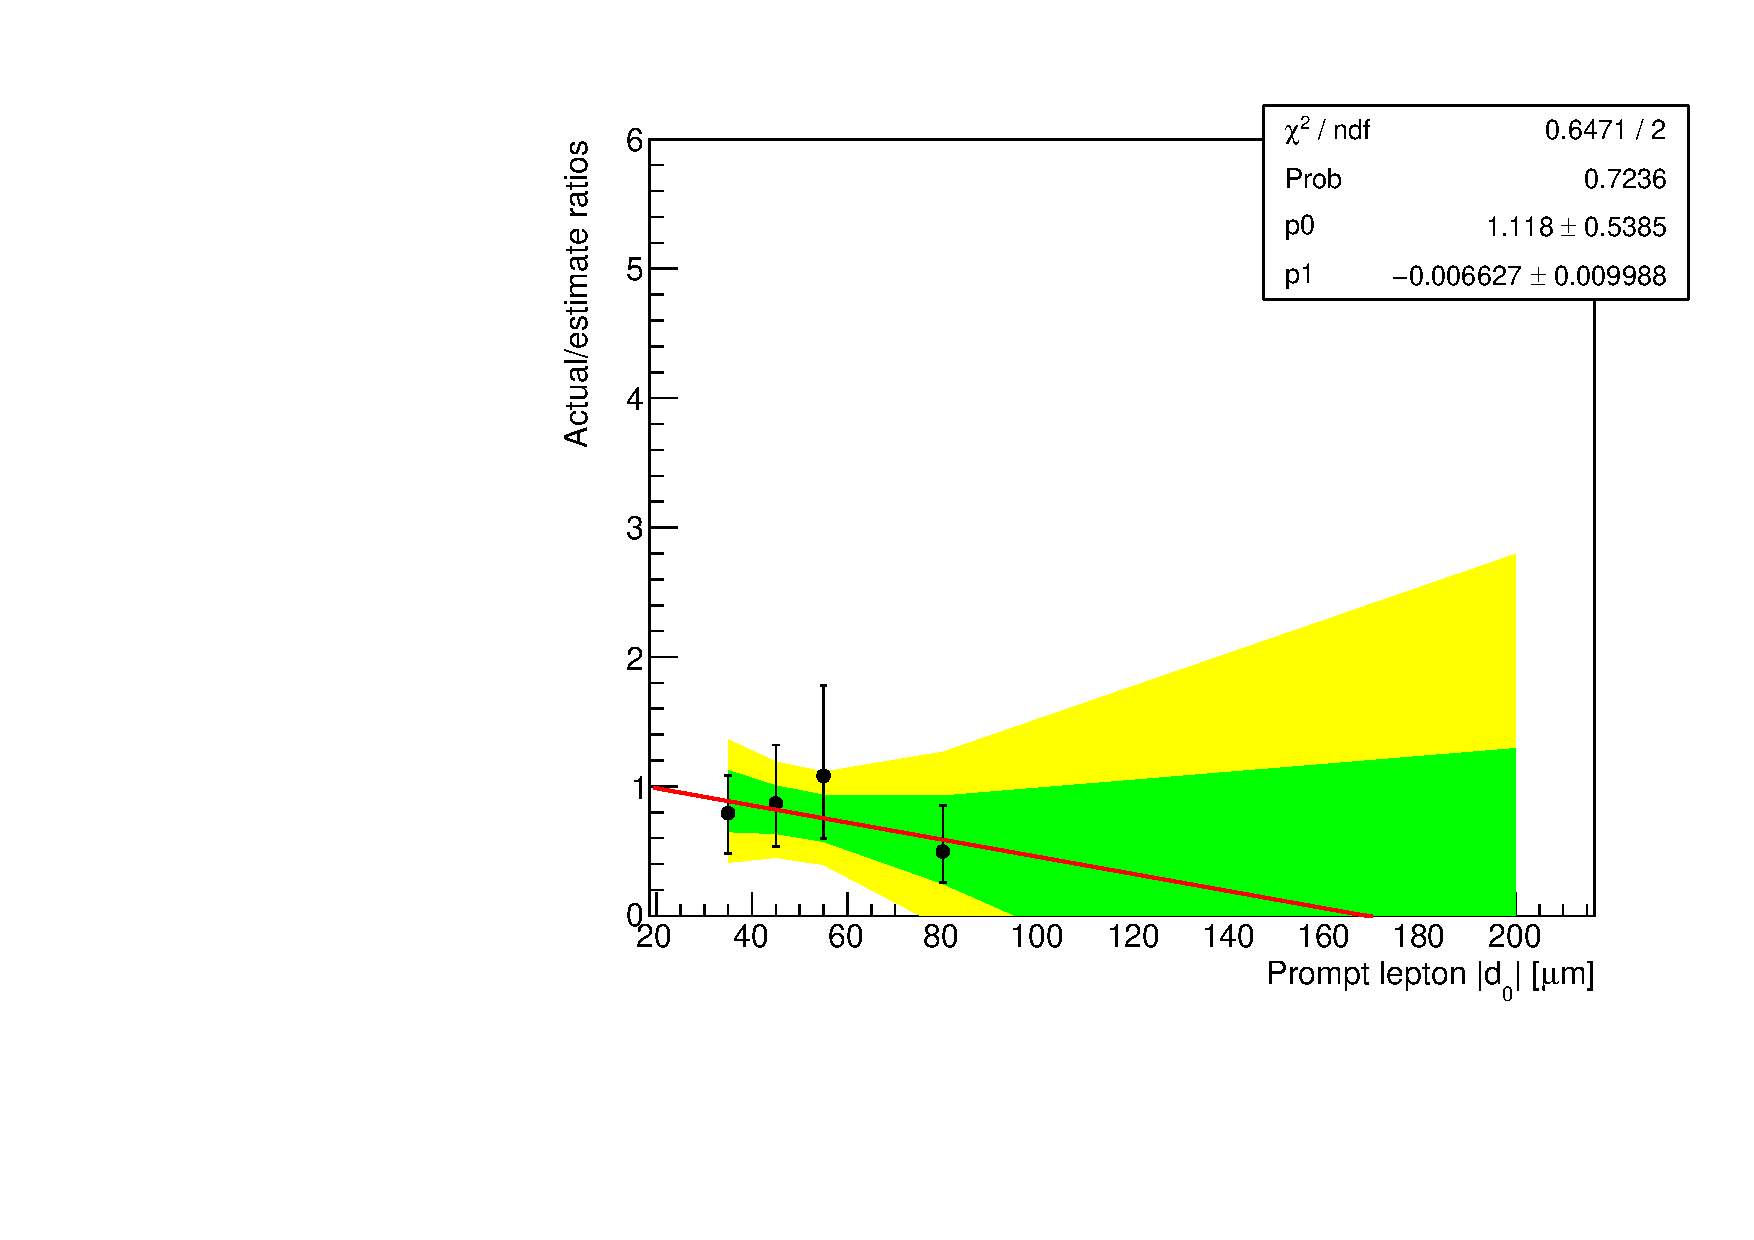
\includegraphics[scale=0.35]{figures/bg/emu_data_2016_displacedMuon_ratiosVsPromptD0.pdf}
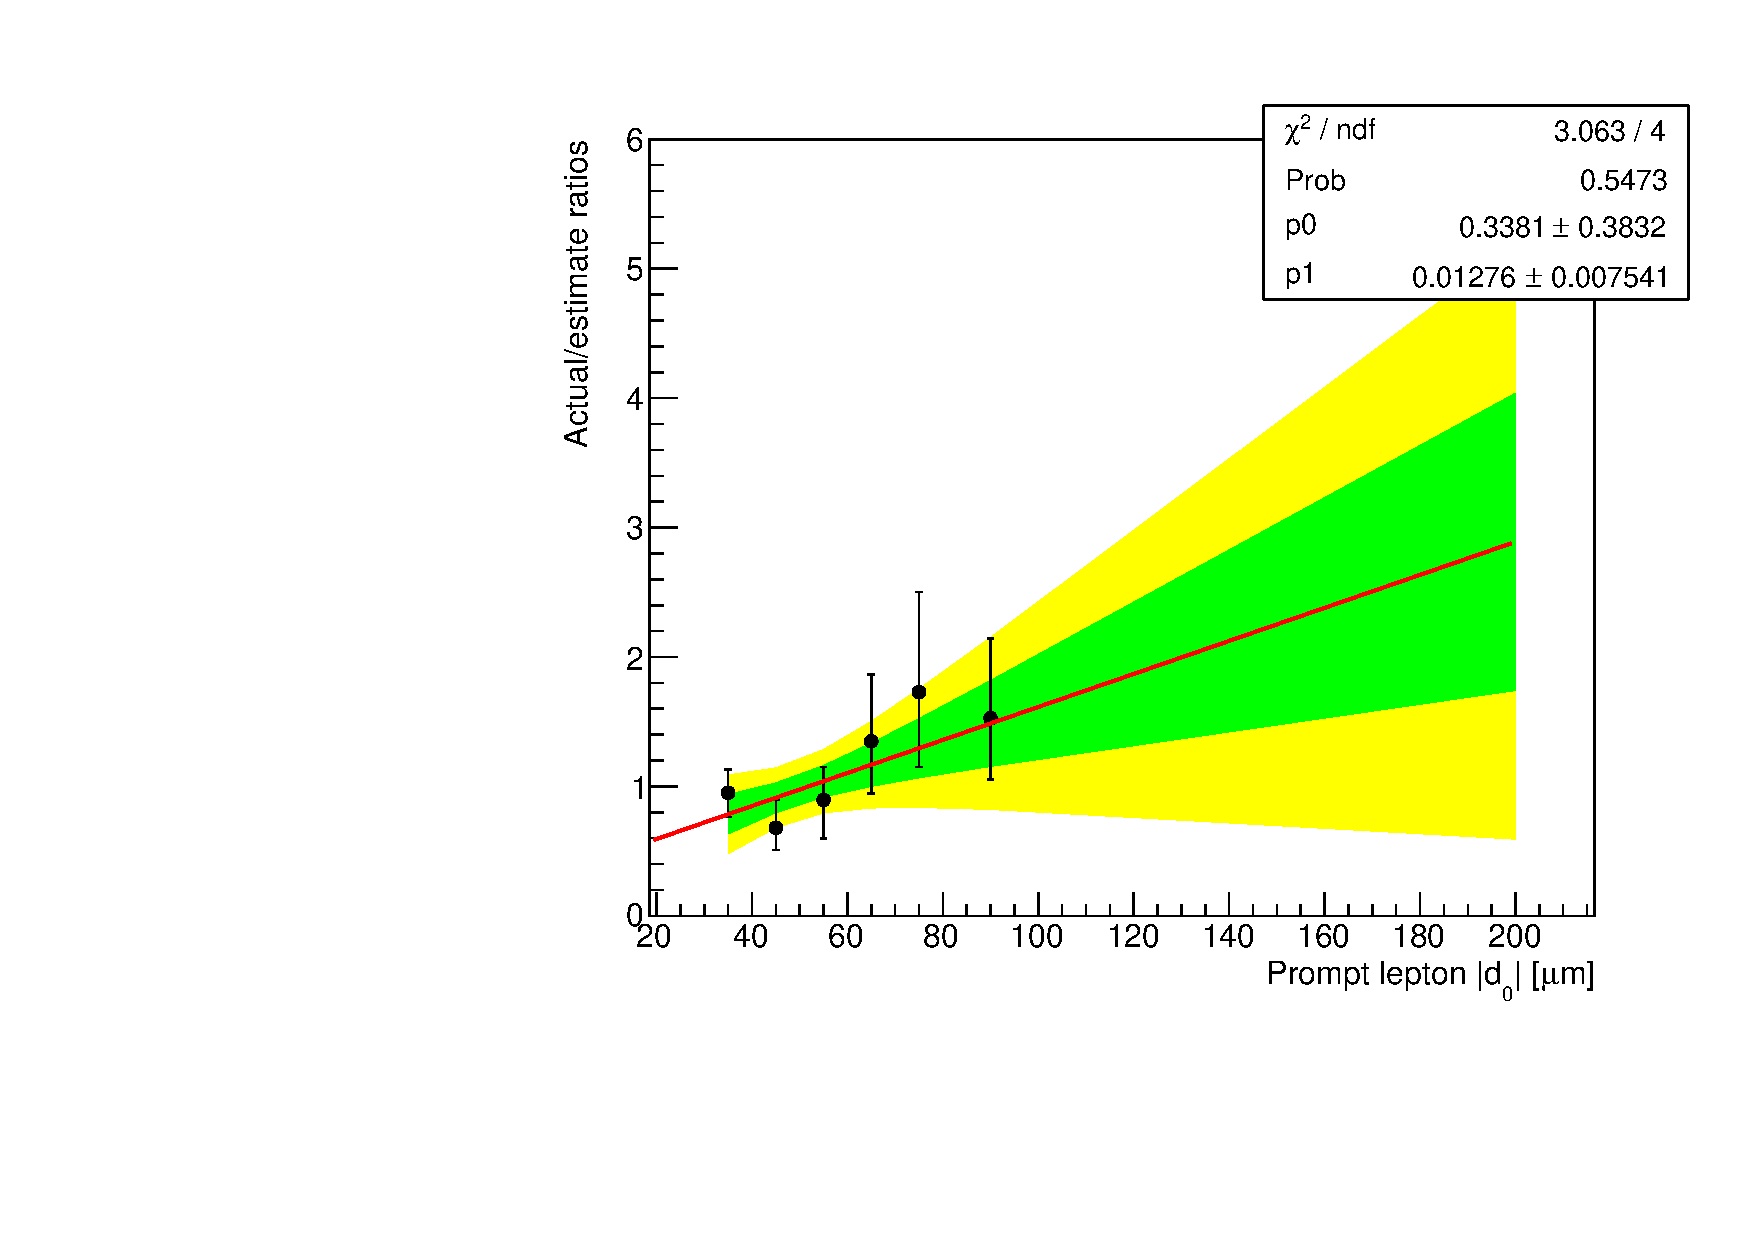
\includegraphics[scale=0.35]{figures/bg/emu_data_2017_2018_displacedMuon_ratiosVsPromptD0.pdf}
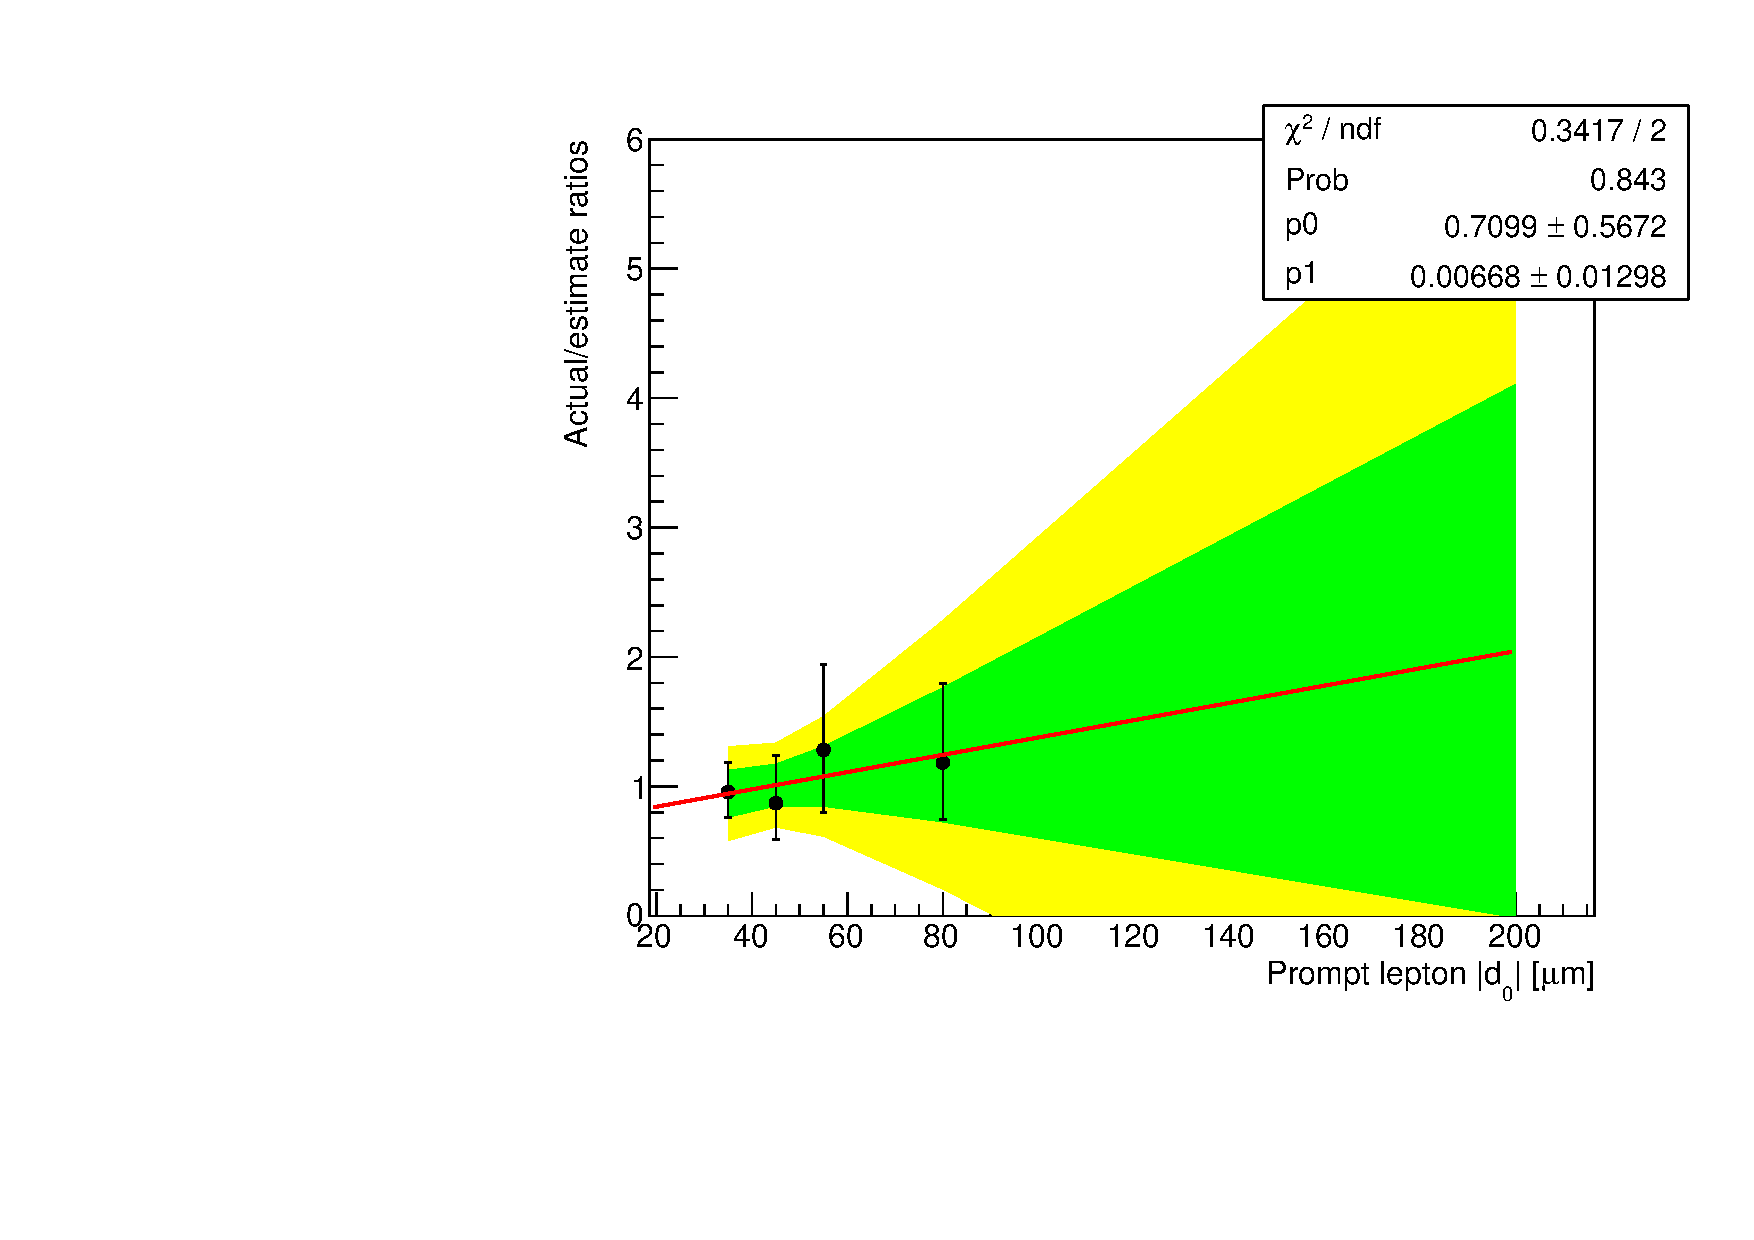
\includegraphics[scale=0.35]{figures/bg/emu_data_2016_displacedElectron_ratiosVsPromptD0.pdf}
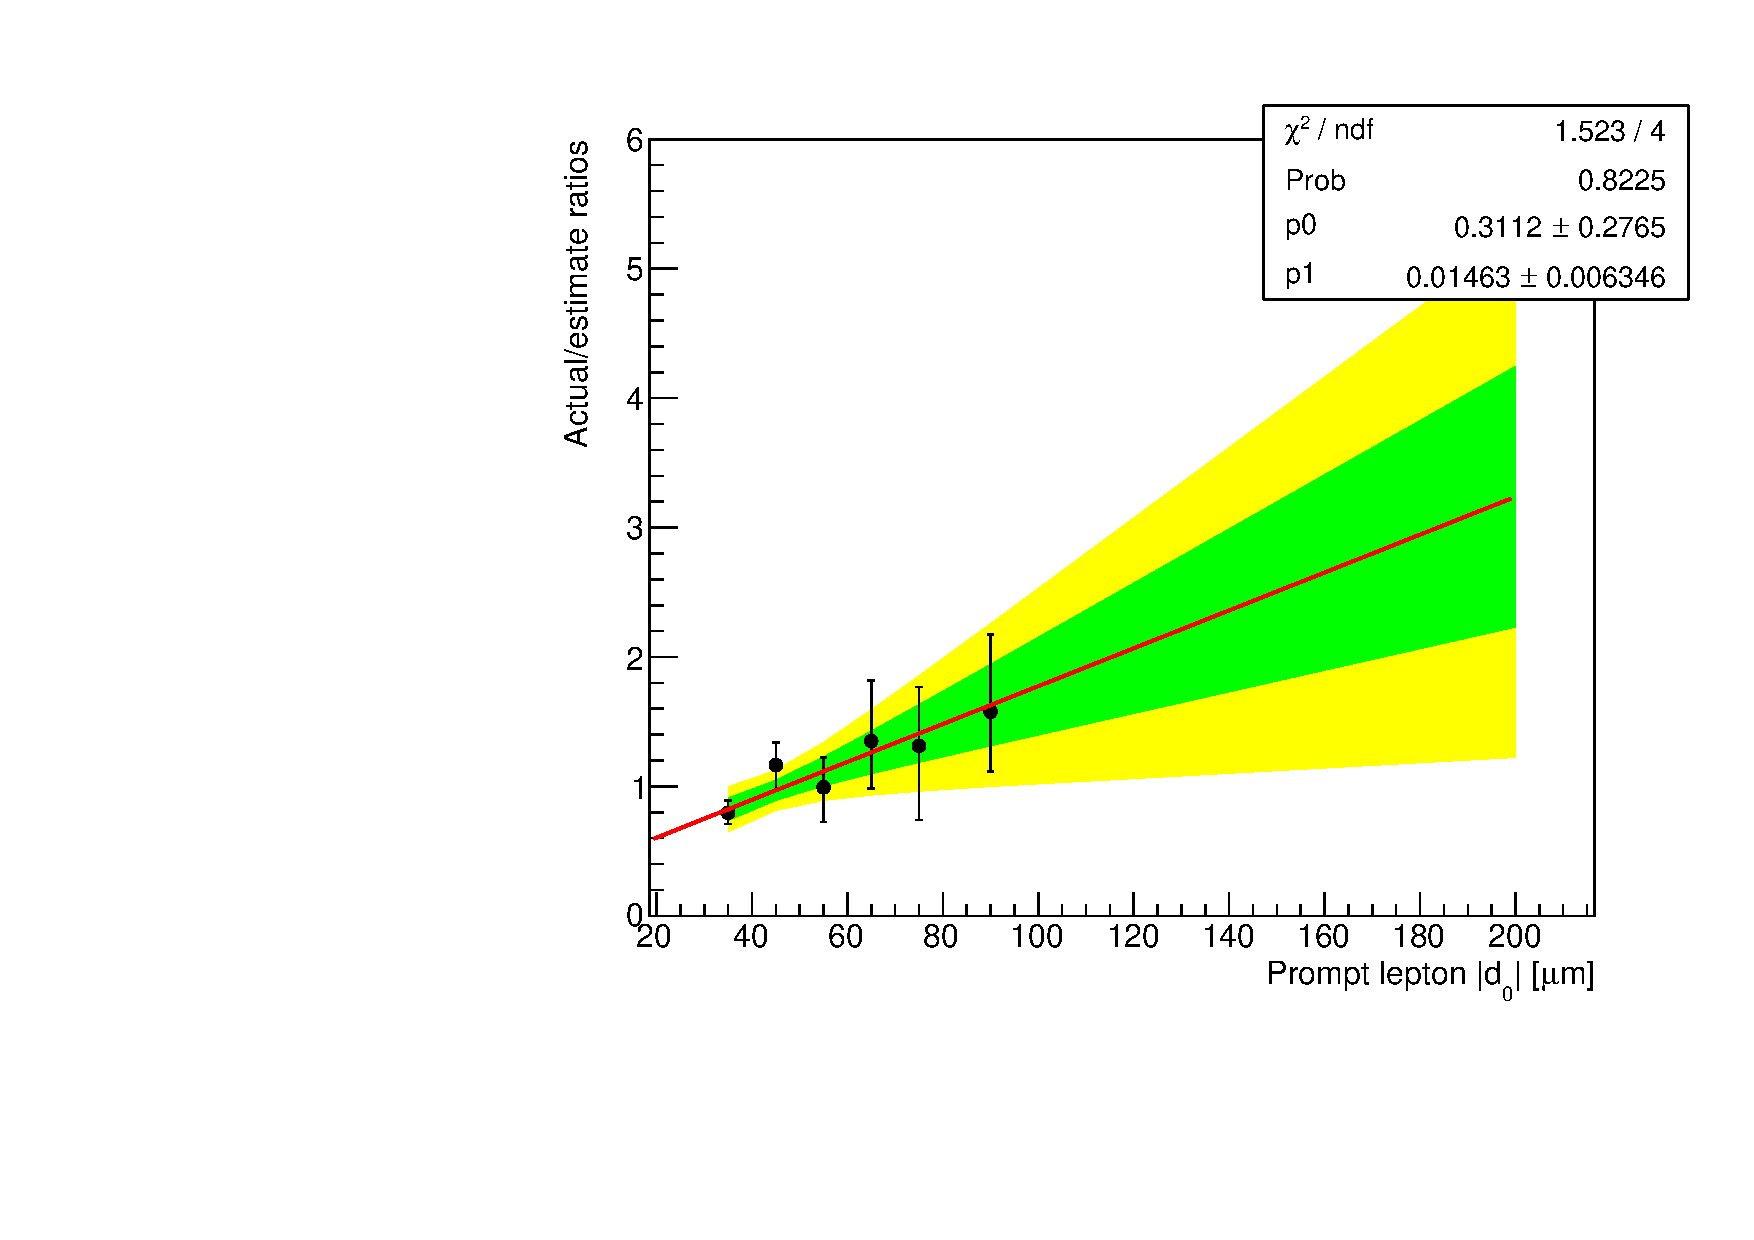
\includegraphics[scale=0.35]{figures/bg/emu_data_2017_2018_displacedElectron_ratiosVsPromptD0.pdf}
\caption{Background estimation closure tests in data, in the one-prompt (20--100\mum)/one-displaced (100-500\mum) sidebands, in the $\Pe\Pgm$ channel. The prompt leading electron/ displaced leading muon sideband is shown in the upper row, and the prompt leading muon/ displaced leading electron sideband is shown in the lower row. The plots on the left show the results for 2016 data, and the plots on the right are for combined 2017 and 2018 data. The plots show the ratio of the actual to the estimated number of events as a function of the prompt lepton \ad. The data are fitted with a straight line, where the slope and y-intercept are allowed to vary. The $1\sigma$ and $2\sigma$ confidence intervals are shown in the green and yellow bands, respectively.}
\label{100to500um_fits_emu}
\end{figure}


\begin{figure}[hbtp]
\centering
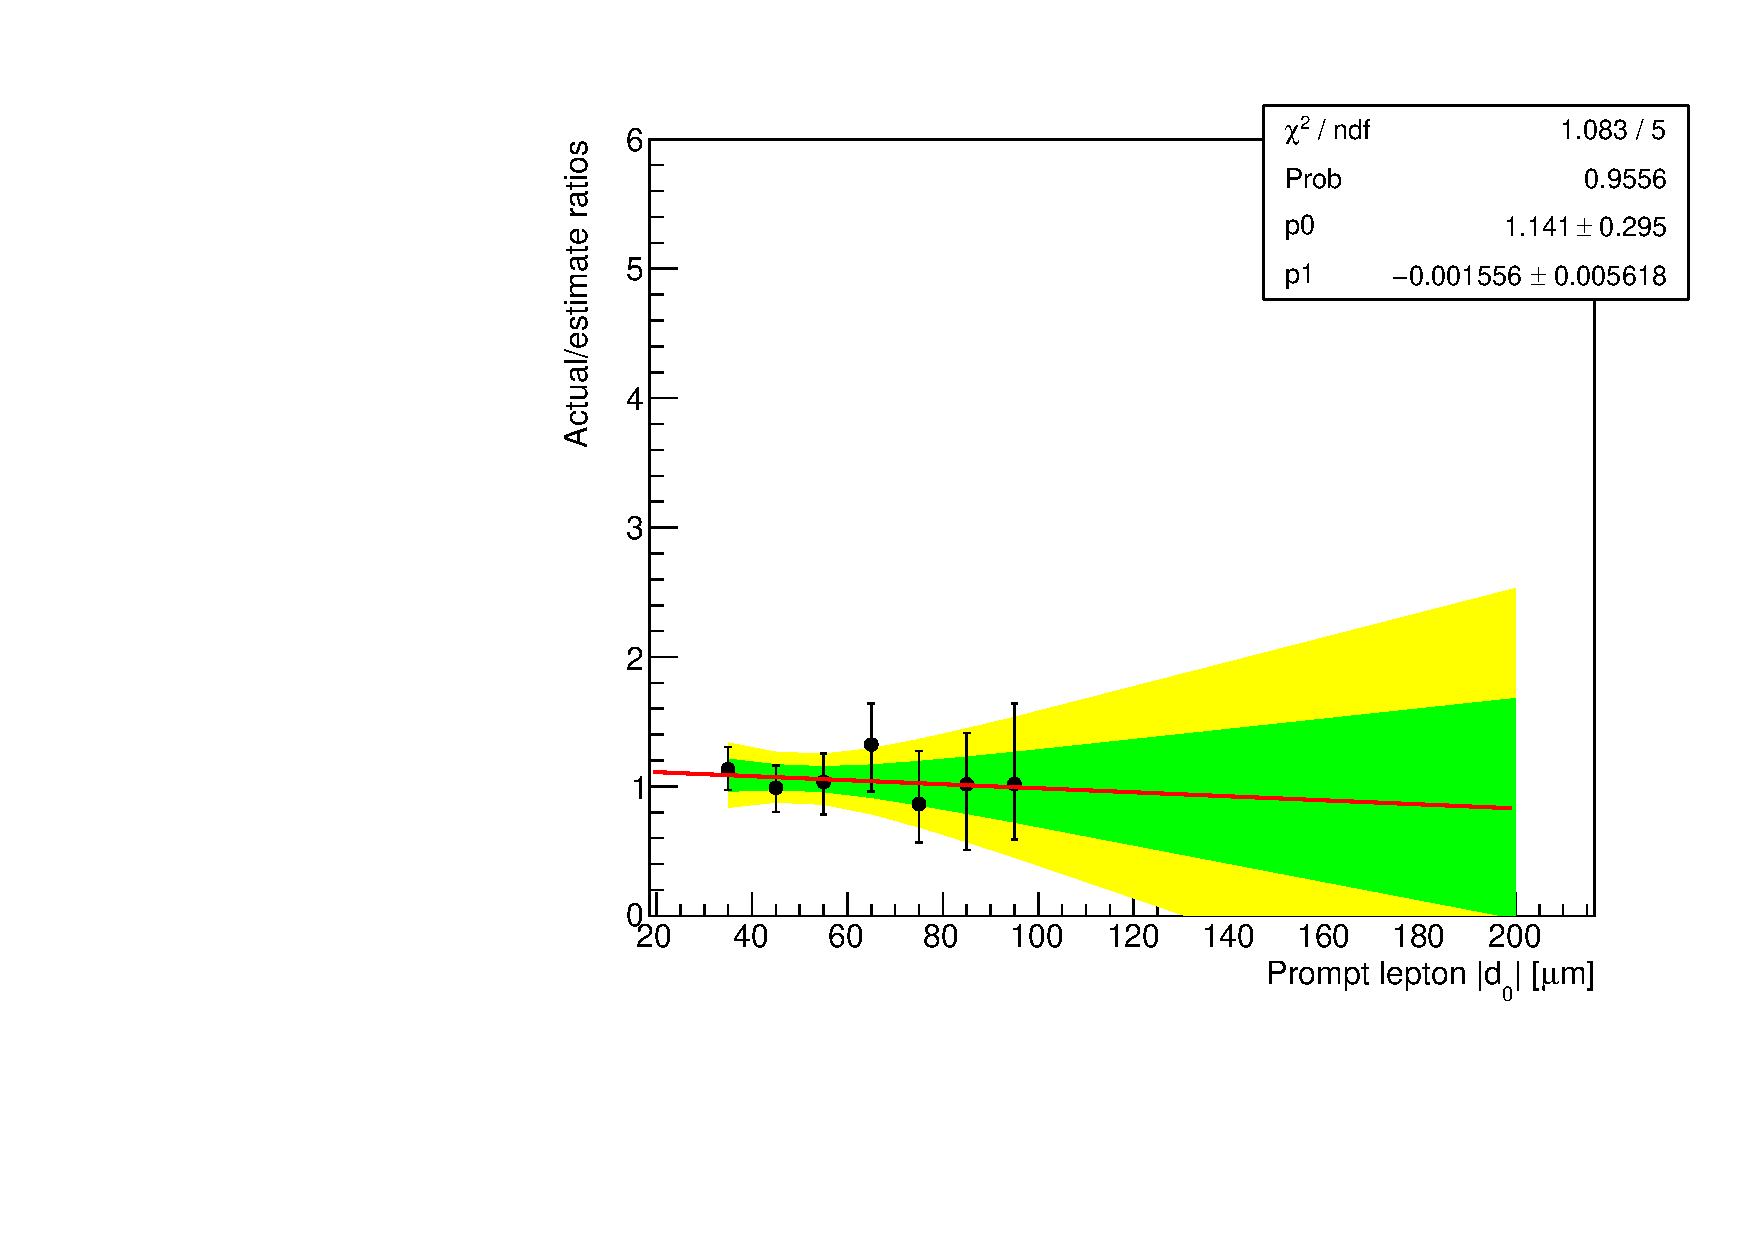
\includegraphics[scale=0.35]{figures/bg/ee_data_2016_displacedSubleading_ratiosVsPromptD0.pdf}
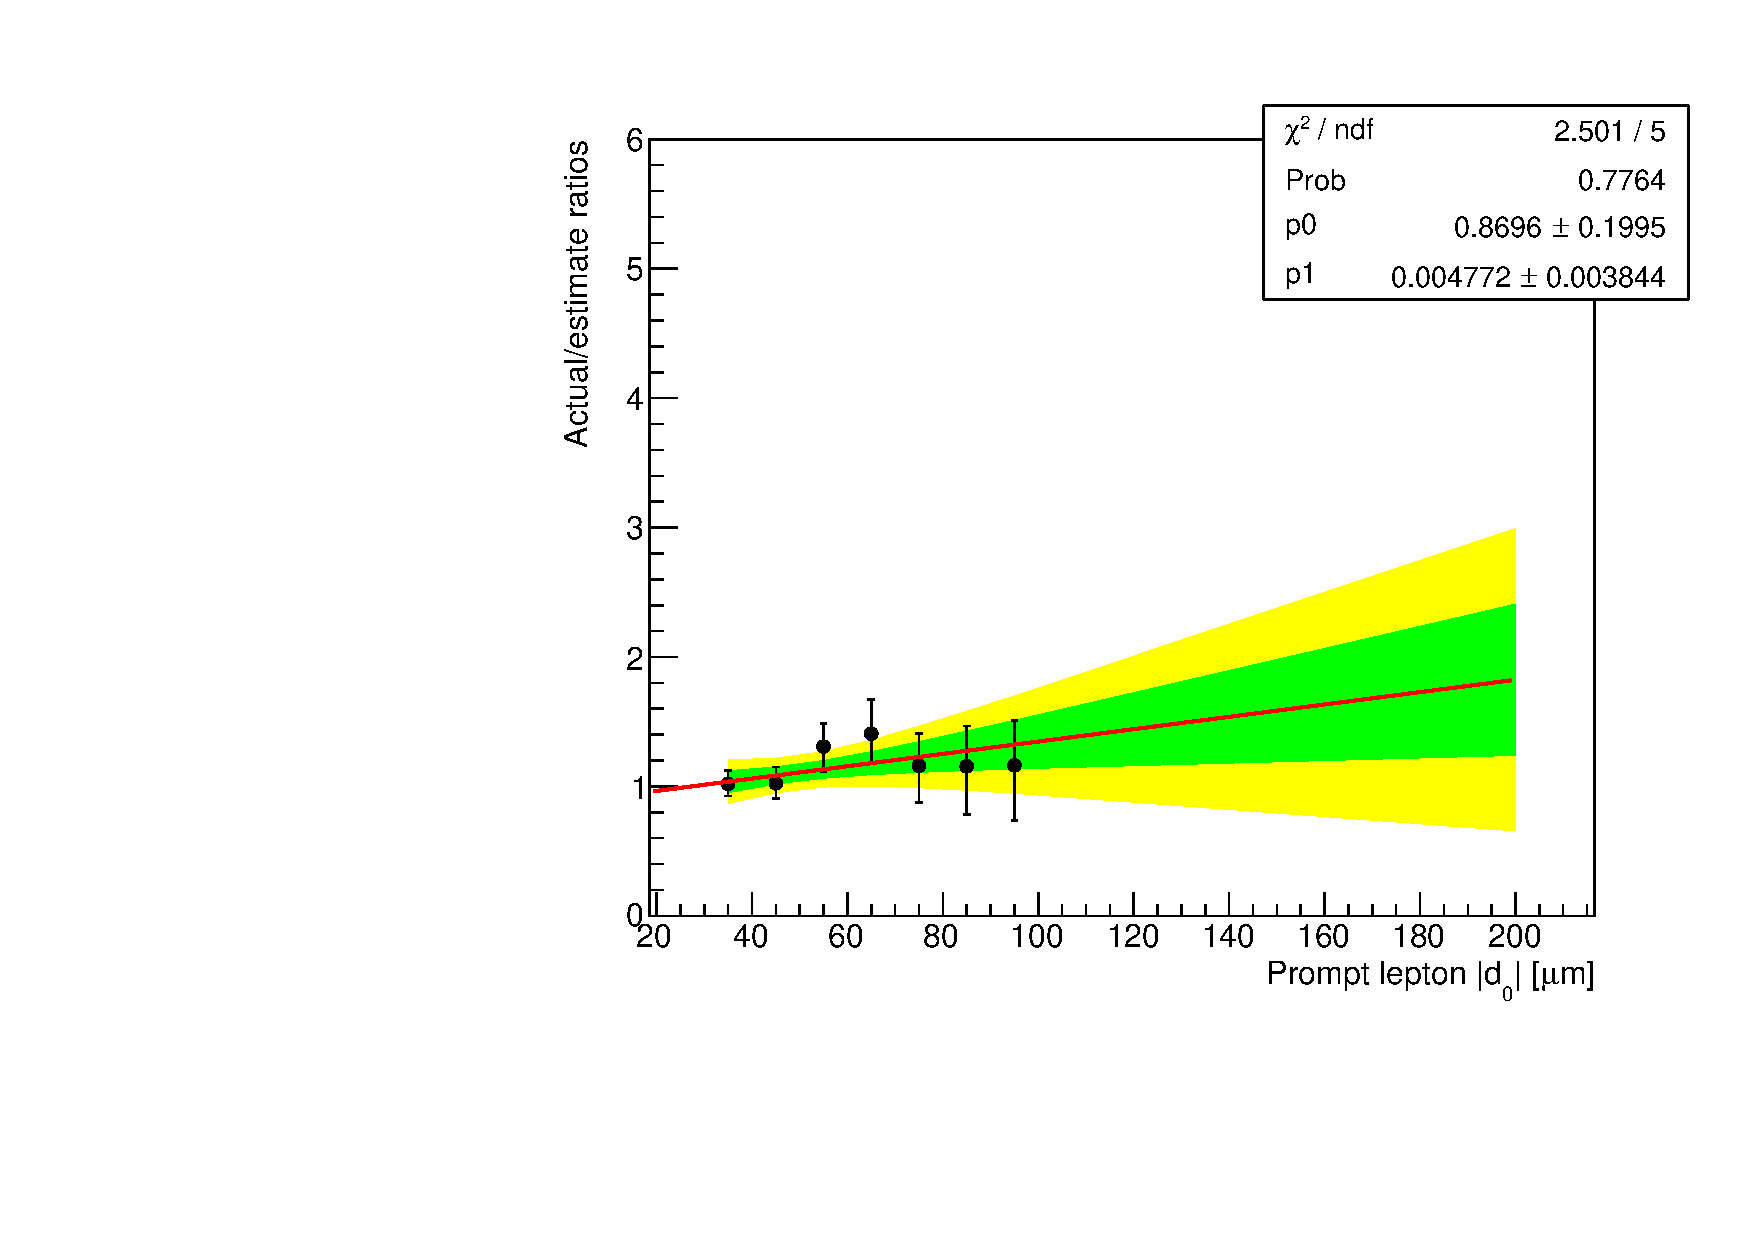
\includegraphics[scale=0.35]{figures/bg/ee_data_2017_2018_displacedSubleading_ratiosVsPromptD0.pdf}
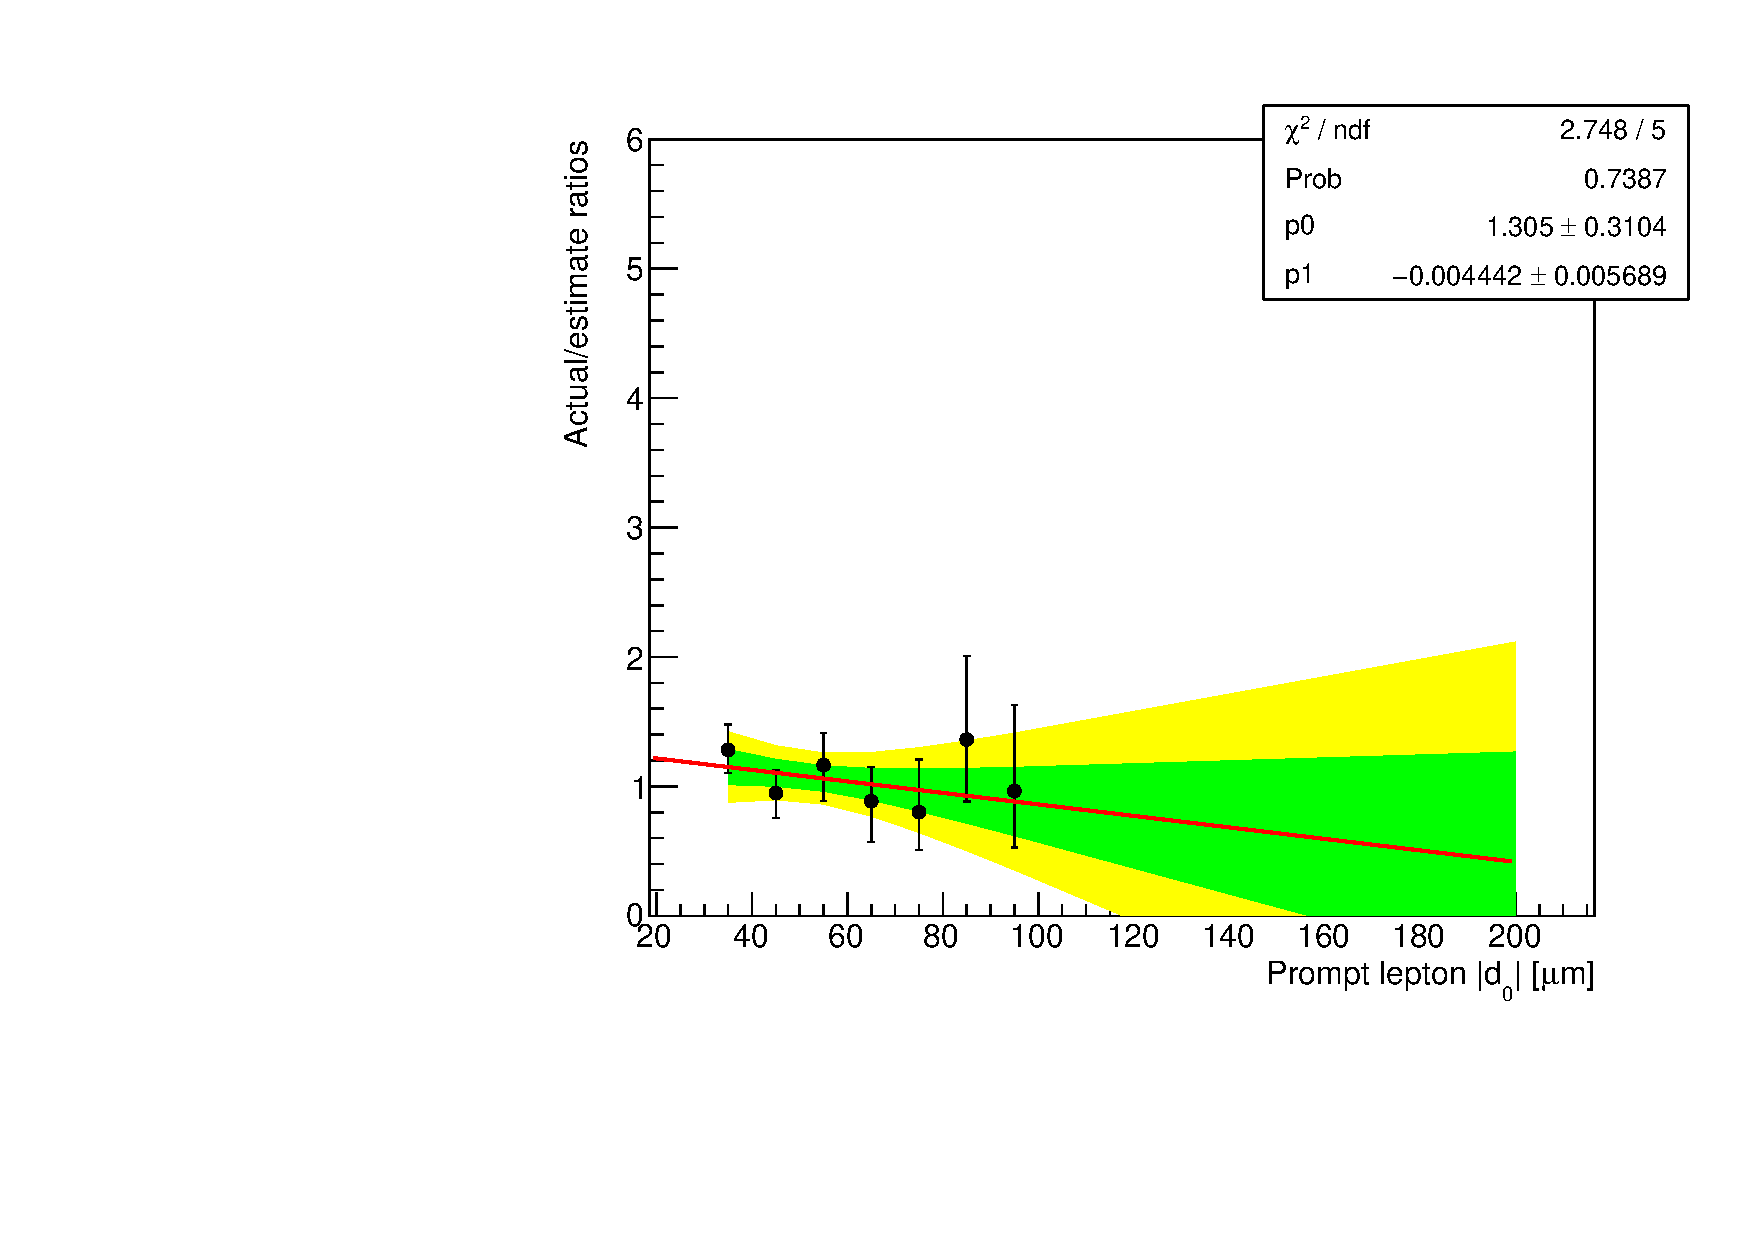
\includegraphics[scale=0.35]{figures/bg/ee_data_2016_displacedLeading_ratiosVsPromptD0.pdf}
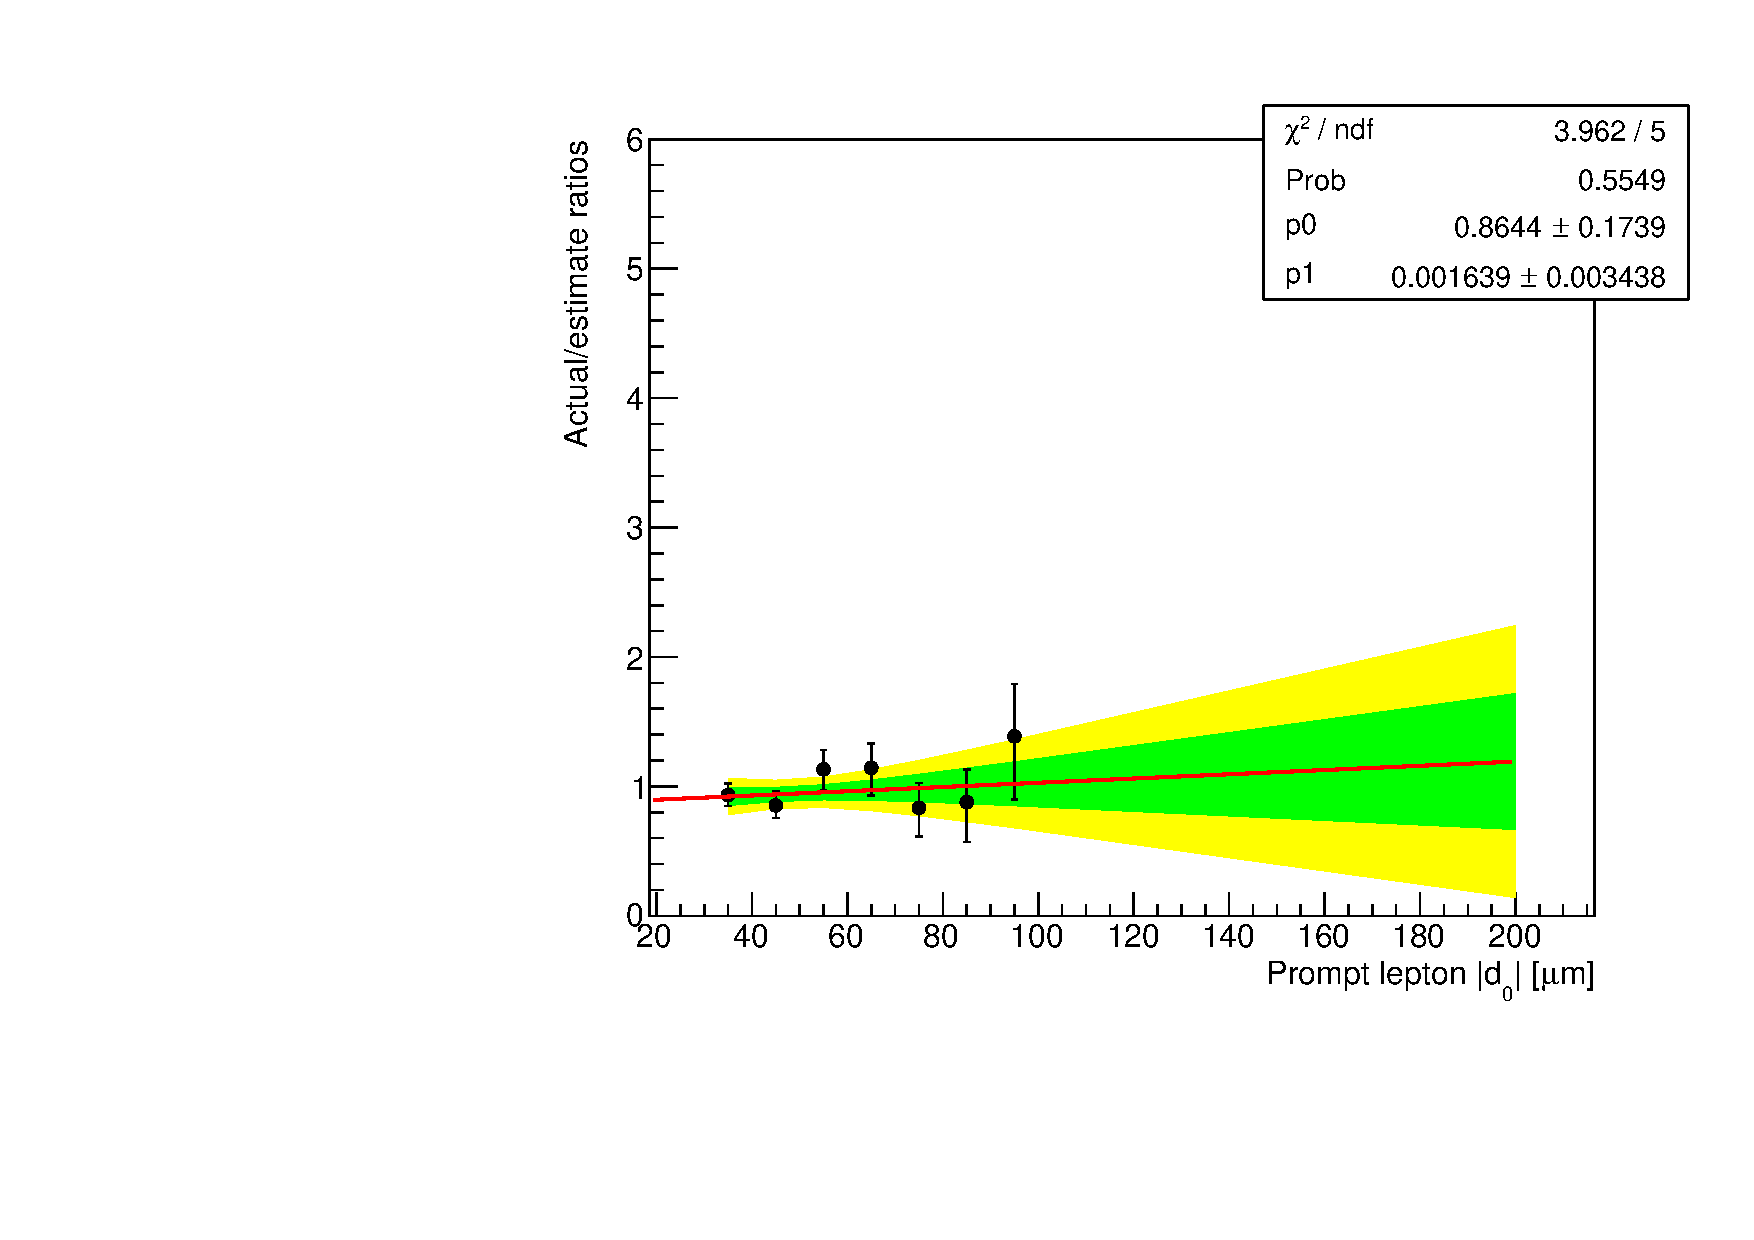
\includegraphics[scale=0.35]{figures/bg/ee_data_2017_2018_displacedLeading_ratiosVsPromptD0.pdf}
\caption{Background estimation closure tests in data, in the one-prompt (20--100\mum)/one-displaced (100-500\mum) sidebands, in the $\Pe\Pe$ channel. The prompt leading electron/ displaced subleading electron sideband is shown in the upper row, and the prompt subleading electron/ displaced leading electron sideband is shown in the lower row. The plots on the left show the results for 2016 data, and the plots on the right are for combined 2017 and 2018 data. The plots show the ratio of the actual to the estimated number of events as a function of the prompt lepton \ad. The data are fitted with a straight line, where the slope and y-intercept are allowed to vary. The $1\sigma$ and $2\sigma$ confidence intervals are shown in the green and yellow bands, respectively.}
\label{100to500um_fits_ee}
\end{figure}


\begin{figure}[hbtp]
\centering
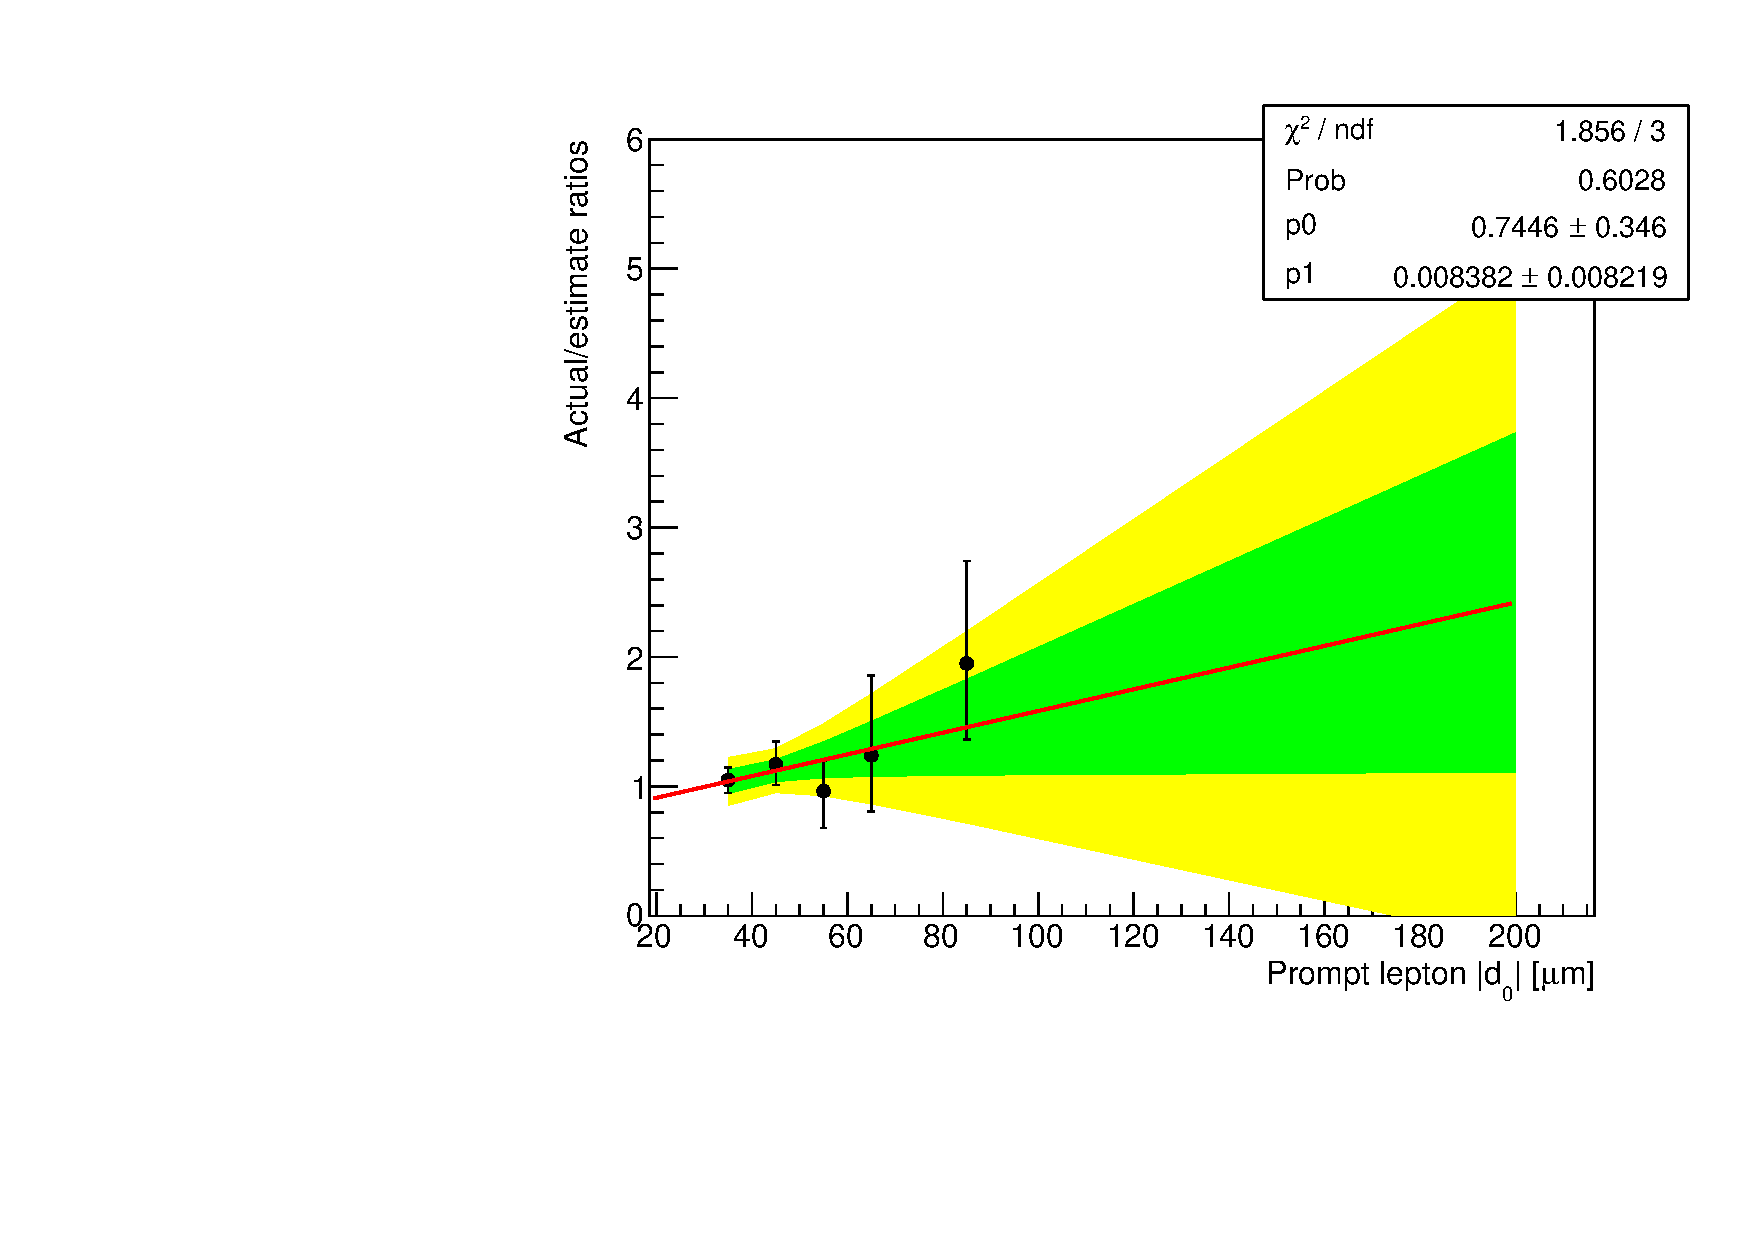
\includegraphics[scale=0.35]{figures/bg/mumu_data_2016_displacedSubleading_ratiosVsPromptD0.pdf}
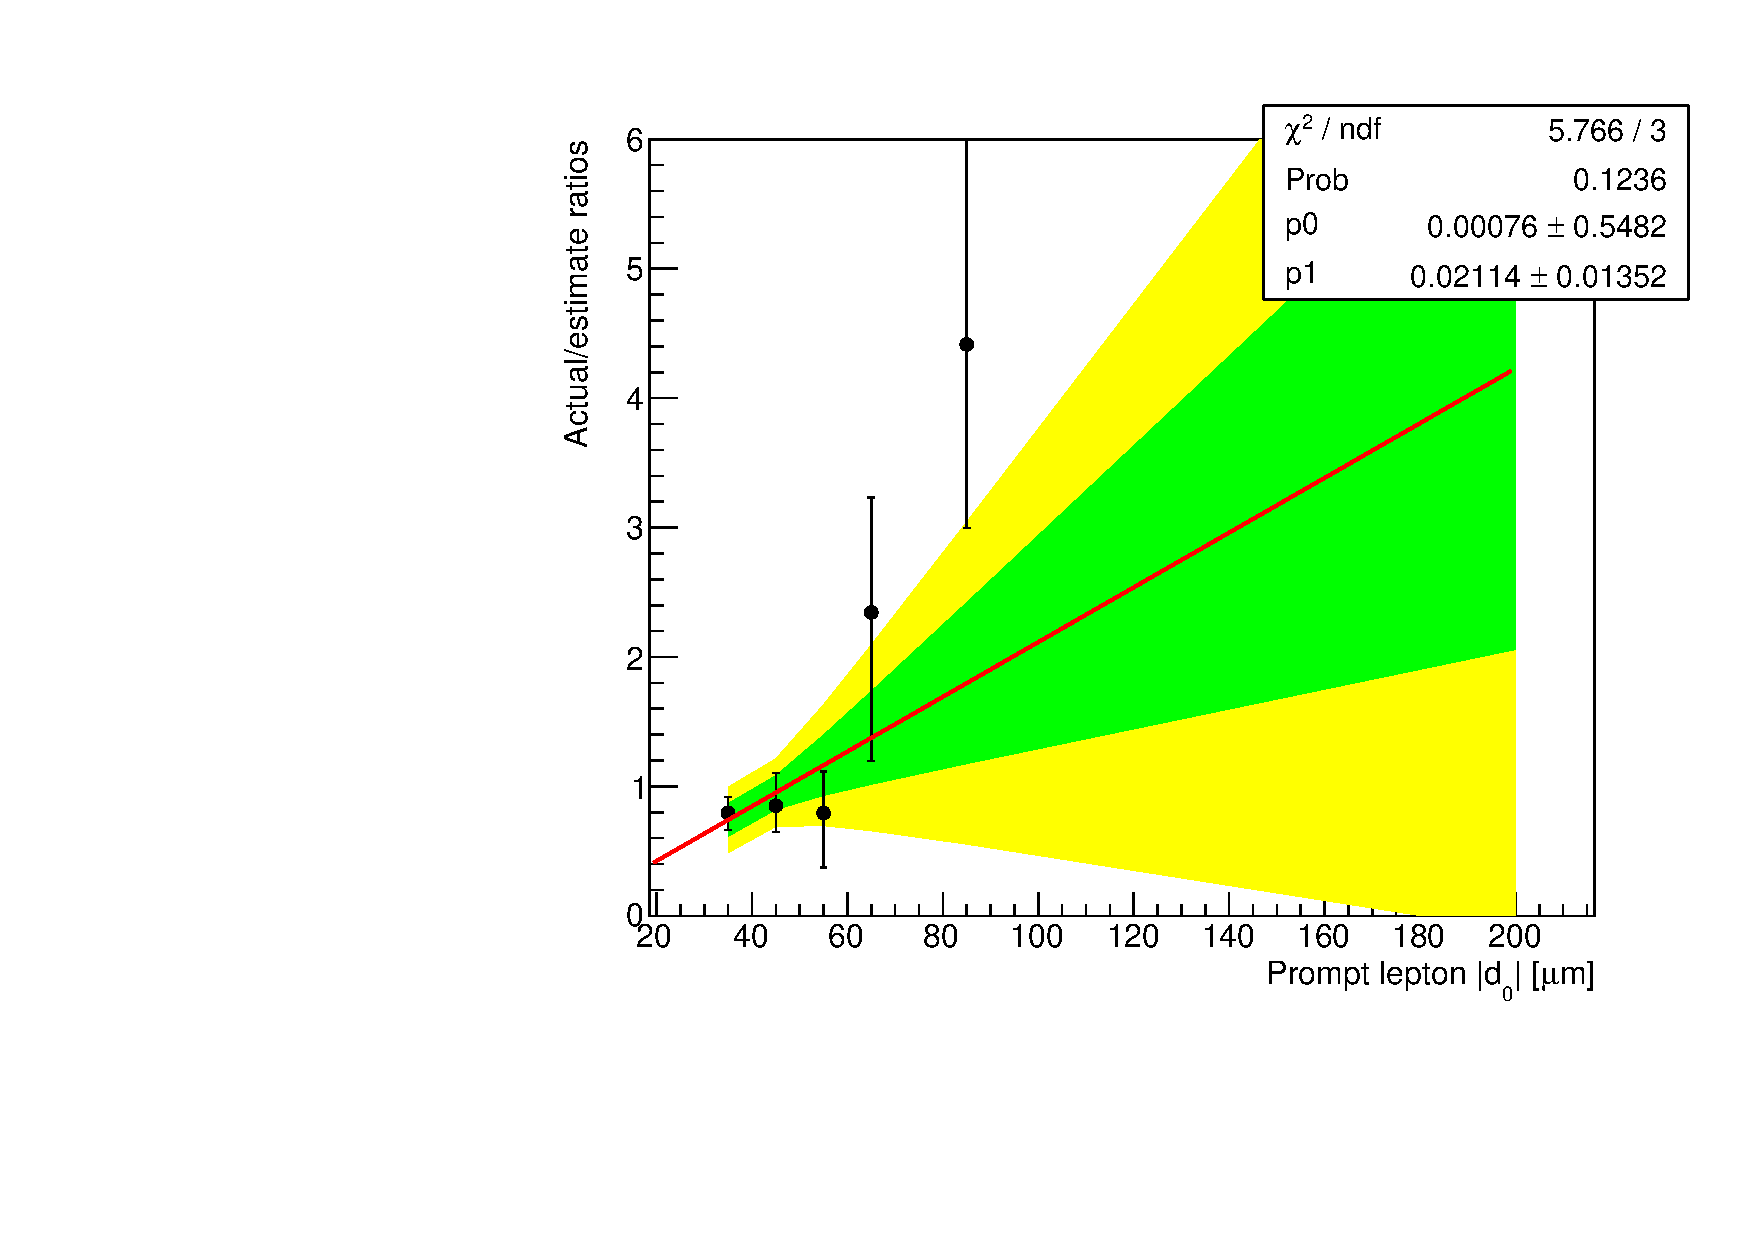
\includegraphics[scale=0.35]{figures/bg/mumu_data_2017_2018_displacedSubleading_ratiosVsPromptD0.pdf}
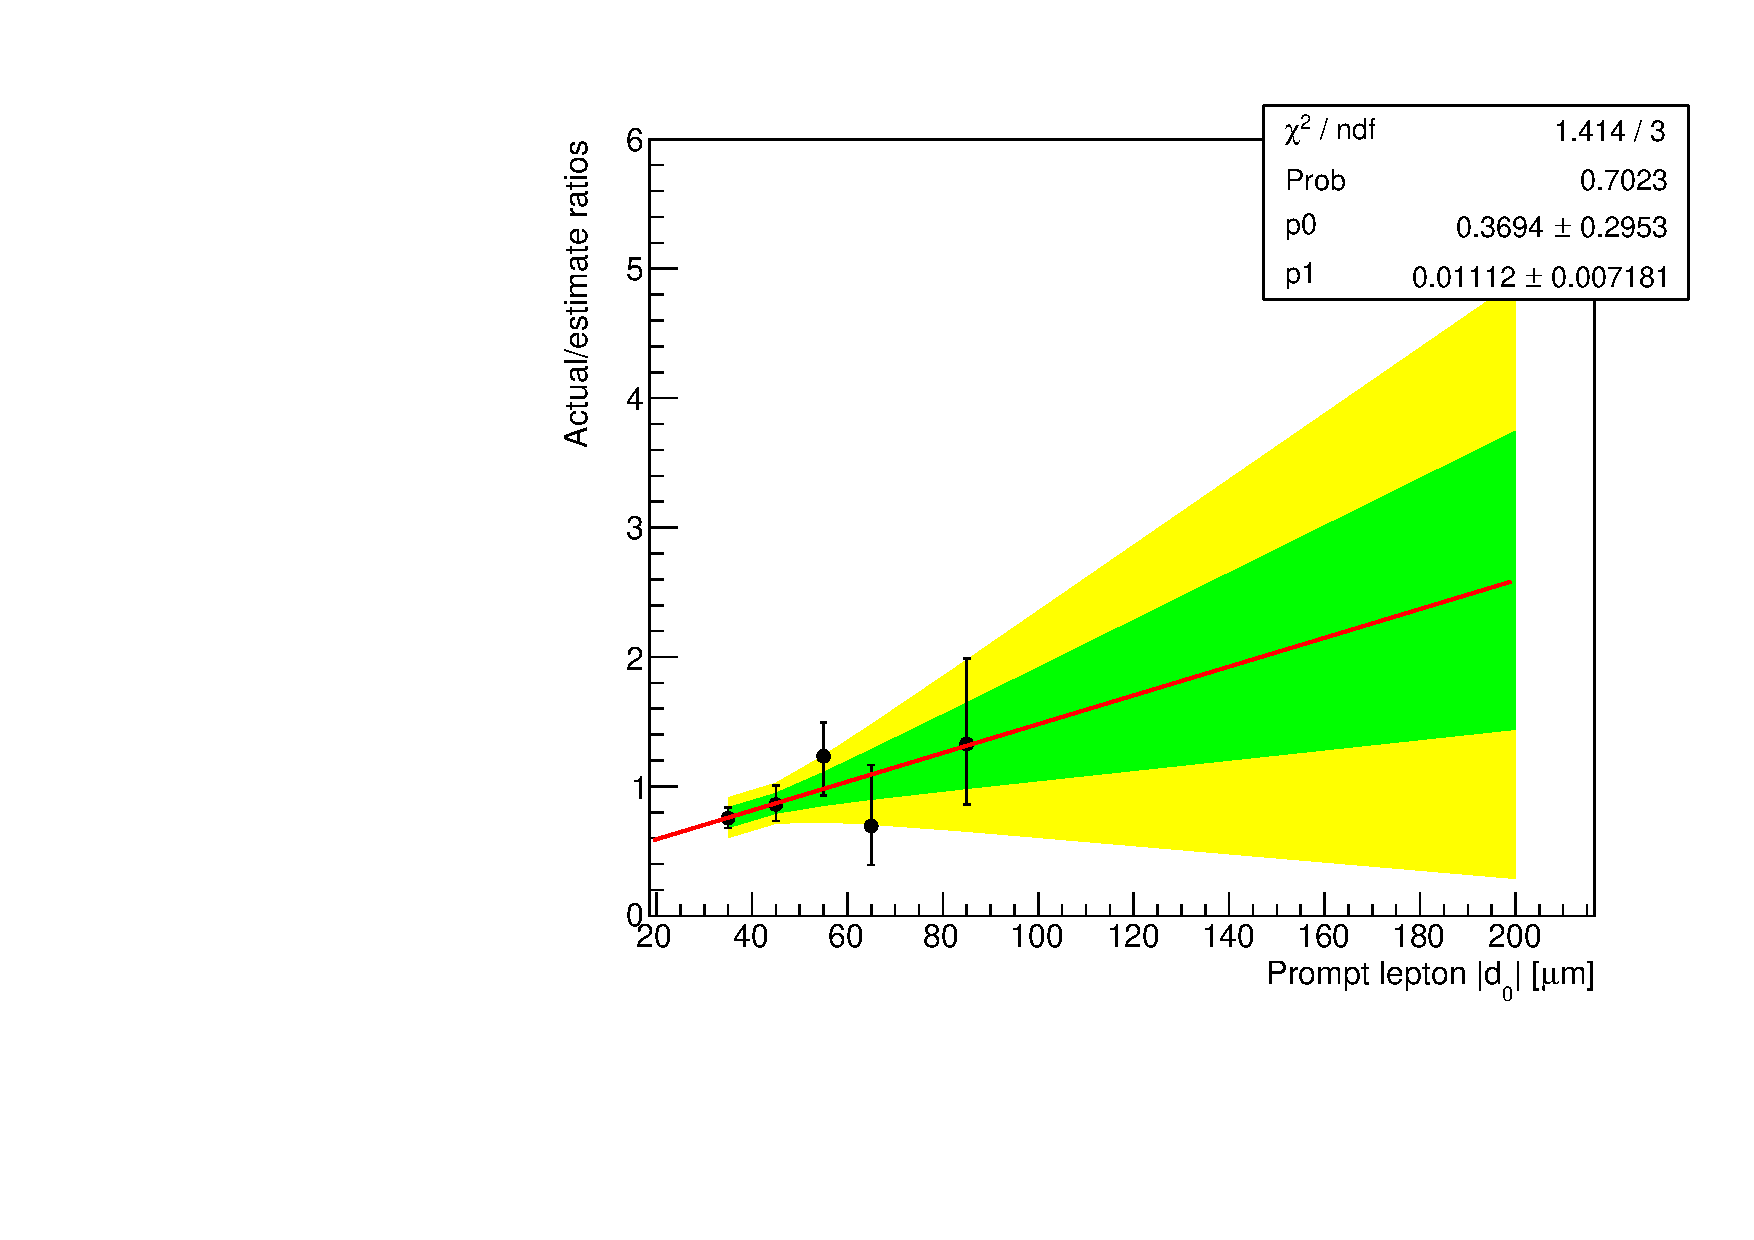
\includegraphics[scale=0.35]{figures/bg/mumu_data_2016_displacedLeading_ratiosVsPromptD0.pdf}
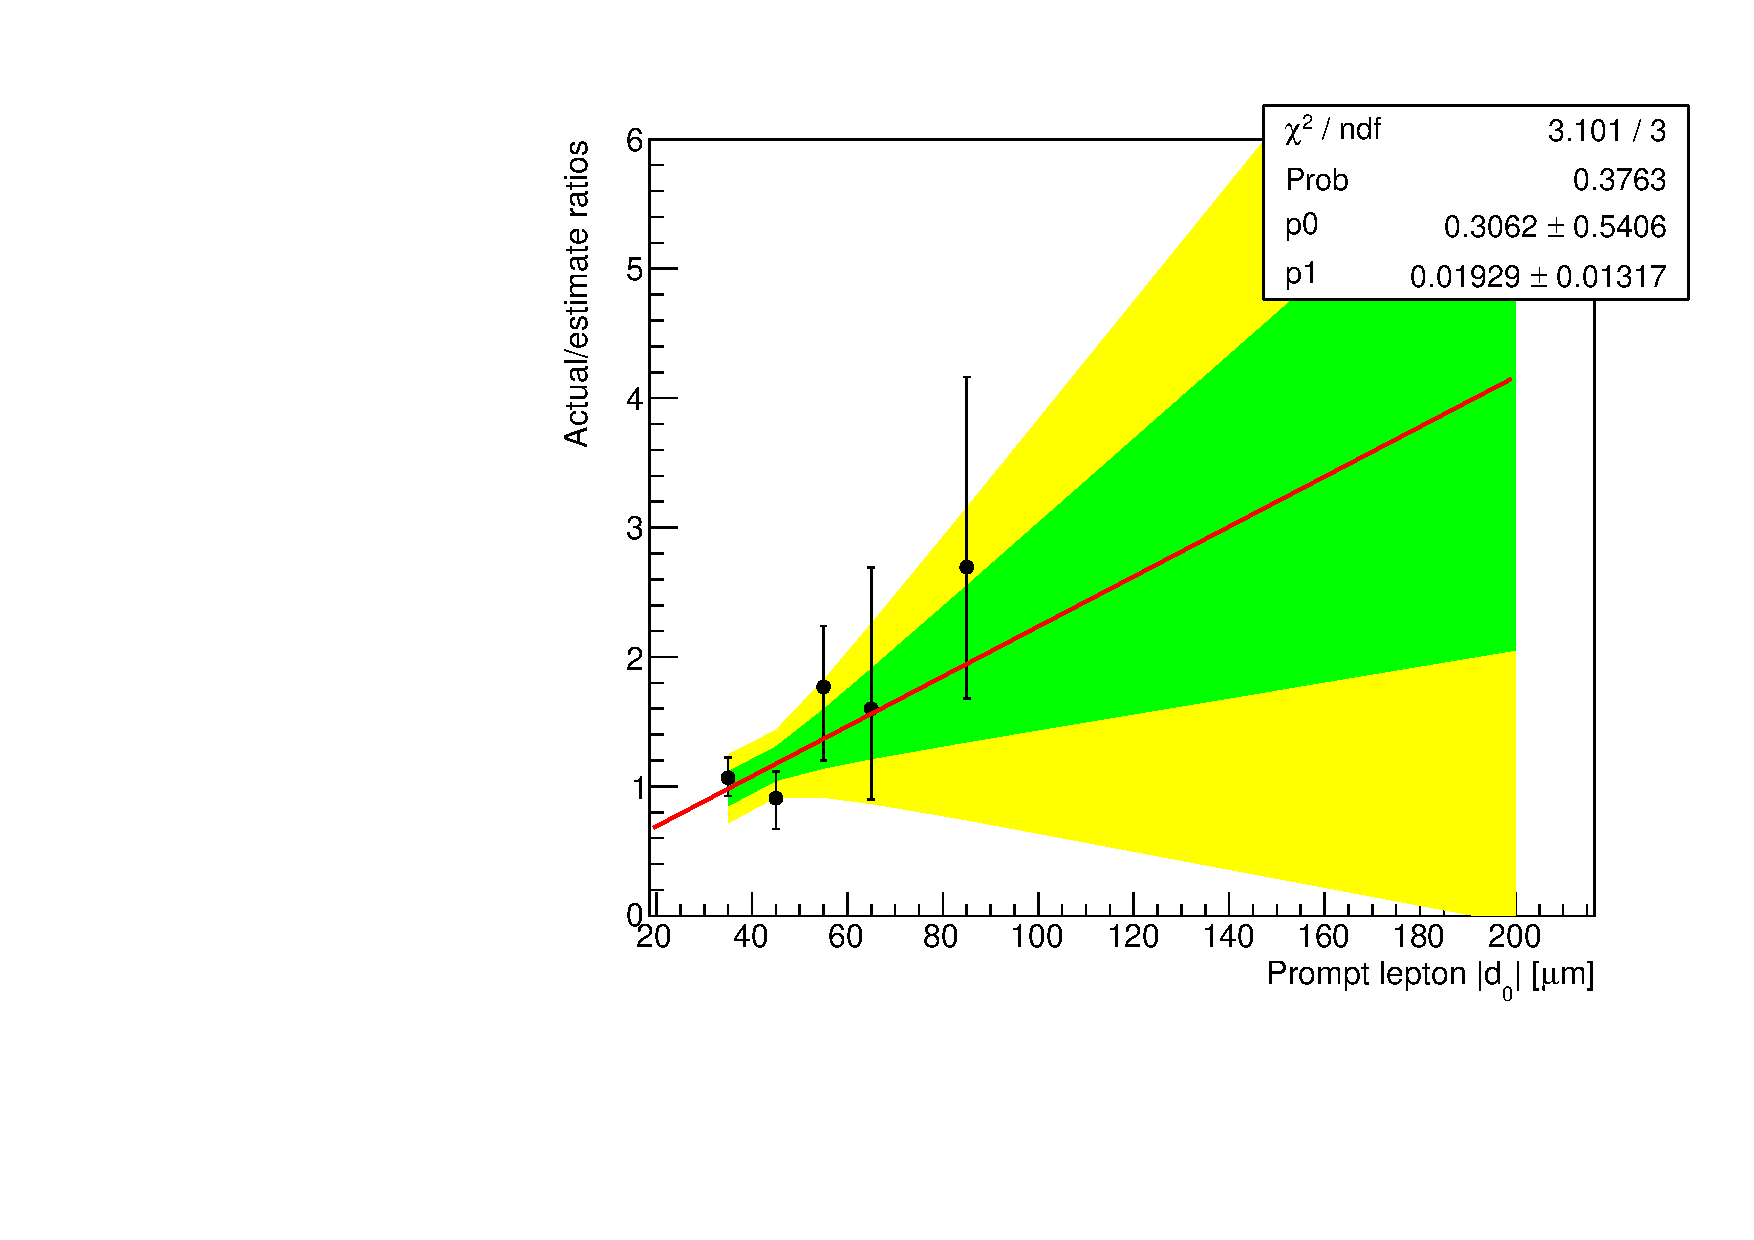
\includegraphics[scale=0.35]{figures/bg/mumu_data_2017_2018_displacedLeading_ratiosVsPromptD0.pdf}
\caption{Background estimation closure tests in data, in the one-prompt (20--100\mum)/one-displaced (100-500\mum) sidebands, in the $\Pgm\Pgm$ channel. The prompt leading muon/ displaced subleading muon sideband is shown in the upper row, and the prompt subleading muon/ displaced leading muon sideband is shown in the lower row. The plots on the left show the results for 2016 data, and the plots on the right are for combined 2017 and 2018 data. The plots show the ratio of the actual to the estimated number of events as a function of the prompt lepton \ad. The data are fitted with a straight line, where the slope and y-intercept are allowed to vary. The $1\sigma$ and $2\sigma$ confidence intervals are shown in the green and yellow bands, respectively.}
\label{100to500um_fits_mumu}
\end{figure}